\documentclass[fontsize=12pt, paper=a4]{scrlttr2}

% MUST SET english OPTION!!
\usepackage[english]{babel}
\usepackage{graphicx} 
\usepackage{url}
\usepackage{fullpage}
\usepackage{pdfpages}
%\usepackage{lineno}
%\linenumbers

% Dont forget to read the KOMA-Script documentation, scrguien.pdf

\setkomavar{fromname}{Solomon Messing} % your name
\setkomavar{fromaddress}{Facebook Data Science\\
1 Hacker Way\\ 
Menlo Park, CA 94025}

\setkomavar{signature}{} % printed after the \closing
\renewcommand{\raggedsignature}{\raggedright} % make the signature ragged right

% Custom options:
\KOMAoptions{firsthead=false}
\makeatletter
\@setplength{backaddrheight}{0pt}
\@setplength{refvpos}{8cm}
\makeatother\makeatother

%\setkomavar{subject}{Politics and Data Science Search} % subject of the letter
\date{September 15, 2014}

\begin{document}

% A little extra room :)
\enlargethispage{6\baselineskip}

\begin{letter}{Professor John T. Scott\\
469 Kerr Hall\\
One Shields Ave\\
Davis, CA\\
95616-8682}

\opening{Dear Professor John T. Scott and Search Committee Members:}  % eg. Hello

I write to express interest in a tenure track position in the Department of Political Science at the University of California, Davis.  I am currently a Data Scientist at Facebook.  % where I employ statistical and computational methods to analyze large data sets and experiments.  
My dissertation ``How Social Influence Shapes the Diffusion of Elite Discourse, Public Opinion, and Participation'' was under the direction of Shanto Iyengar (chair), Simon Jackman, Justin Grimmer, Jeremy Bailenson, and Cliff Nass.

My dissertation examines how social processes shape the interplay between elite opinion and public opinion, using web experiments and machine learning.  Sharing or endorsing elite opinion changes the way a person's friends respond to political discourse, triggering complex evaluations of the sharer's personal attributes, group membership, and the relationship with the sharer.  This not only makes it more likely that she carefully evaluates the discourse, but also changes the \emph{way} she thinks about it.  Furthermore, when she encounters more shared political discourse in social media, she is more likely to hold informed opinions and actually vote.  Rather than ``minimal effects,'' elite ideas delivered personally shape how Americans think and behave in the political sphere.

%I don't the third paragraph is doing what it needs to do
%I don't *think* it is clear that you are not just talking about general changes and not *things* specific to your work
The massive quantity of fine-grained data now available thanks to the emergence of modern web technologies means that we can move beyond case studies and observe these processes at scale, \emph{in situ}.  Hence, my work uses a series of original web-experiments, large-scale behavioral studies of social networks, and analyses of large scale text corpora.  This allows me to estimate \emph{long-term}, ecologically valid causal effects showing how social influence shapes political outcomes.  The result is a rich account of how social influence impacts public opinion and political behavior.  

Related work shows how these processes drive attention. In ``Selective Exposure in an Age of Social Media,'' with Sean Westwood (2012, \emph{Communication Research}), we use a series of experiments to show that social cues drive more attention than partisan cues.  %In ``Friends that Matter,'' (under revision) I show with a web experiment that when close friends recommend an article, people pay closer attention to it.  
In ``Social News in Black and White,'' (under review) I show paradoxically that people attend to content shared those who are racially similar, but provide more positive evaluations of welfare policies after reading articles shared by blacks compared to whites.  

Changes in communication technology favoring personal interactions also have implications for elite-level American politics and policymaking, especially in the realm of representative-constituent communication.  In work with Justin Grimmer and Sean Westwood (2012, \emph{APSR}), we dissociate the effect of \emph{claiming credit} for particularistic spending from that spending itself using  experiments conducted via email and Facebook.  %In contrast to theoretical models of credit allocation, increasing the number of statements cultivates orders of magnitude more support than increasing the dollar amount claimed.  
We build on these findings in our book, \emph{The Impression of Influence}, (\emph{Princeton University Press}), which shows how legislators exploit constituents' limited knowledge of appropriations to get credit for bureaucratic spending over which they have little control.  

Future work in this area will more deeply examine constituent communication, representation and policy-making using data obtained by forging relationships with major social media companies.  I have acquired a data set from Twitter under a pilot test of what is now their data grant program, which comprises every public Twitter communication sent to and from every congressional representative since 2005; with Stanford graduate student Annie Franco, we've also assembled a similar data set at Facebook.  By combining these massive data sets with Justin Grimmer's press release database, we will have an unprecedented archive of representative-constituent communication to continue this work.

My work with web experiments and large behavioral data sets is part of a broader research agenda focused on applying data science to answer substantive questions in political science.  In ``Quantifying Social Media's Political Space,'' (with Robert Bond, Forthcoming, \emph{APSR}), we develop a model to simultaneously estimate the ideology of politicians and their supporters, which is strongly correlated with both DW-NOMINATE and survey measures of ideology.  We plan to expand this project to estimate ideology in a cross-national context.  In ``Bias in the Flesh: Skin Complexion and Stereotype Consistency in Political Campaigns'' (Forthcoming \emph{POQ}) I apply new methods that measure the appearance of skin complexion in digital images to uncover subtle biases in campaign imagery, using observational and experimental designs.  Work in progress uses this measure to examine the relationship between skin complexion and electoral performance among minority candidates.  

My teaching compliments this research agenda.  I teach statistics modules for Facebook's Data Camp and co-taught a course in Udacity's Data Science track, Exploratory Data Analysis.  At Stanford, I created and taught \emph{Political Communication and Social Media}, which teaches scraping and analyses of text-as-data to examine the role of social technologies in modern politics.  I also served as course assistant for Justin Grimmer's \emph{Text as Data}, teaching assistant for Shanto Iyengar's \emph{Campaigns, Voting, Media and Elections}, and two additional social science courses.  I am interested in creating a course on the role of ``big data'' in politics and policy, on which I plan to bring to bear my experience as a practitioner.  

I am enclosing a curriculum vitae, writing sample, and a summary of my research and teaching interests. My letters of recommendation (from Professors Shanto Iyengar, Justin Grimmer, and Simon Jackman) will be forwarded to you separately. Please contact me if I can provide any additional information. I look forward to hearing from you.

\closing{
Sincerely, \\
%\fromsig{\includegraphics[scale=.5]{SigBlue.jpg}} \\
Solomon Messing\\
Facebook Data Science \\
 \url{solomonmessing.wordpress.com}
}

%\includegraphics{SigBlue.jpg}
%\closing{Sincerely, } %eg. Regards
\end{letter}

%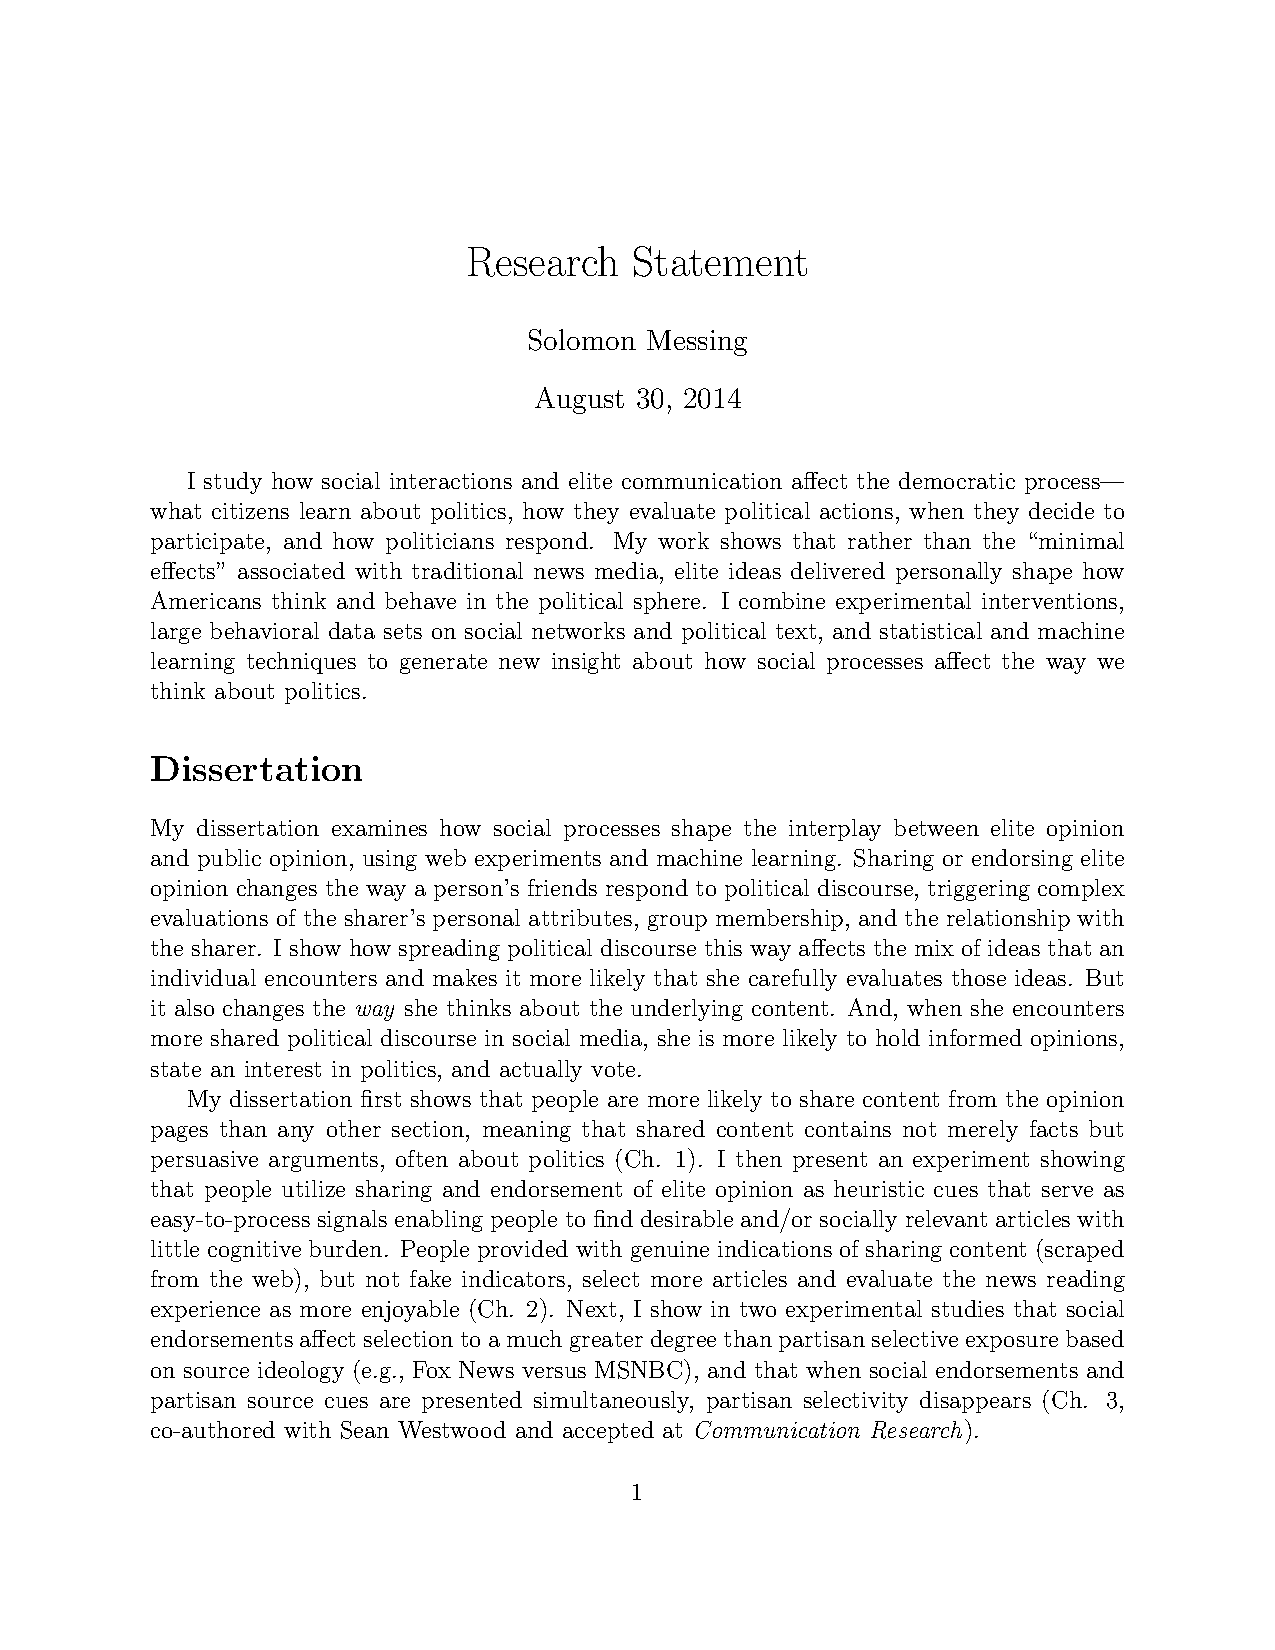
\includepdf[pages={-}]{RS.pdf}
%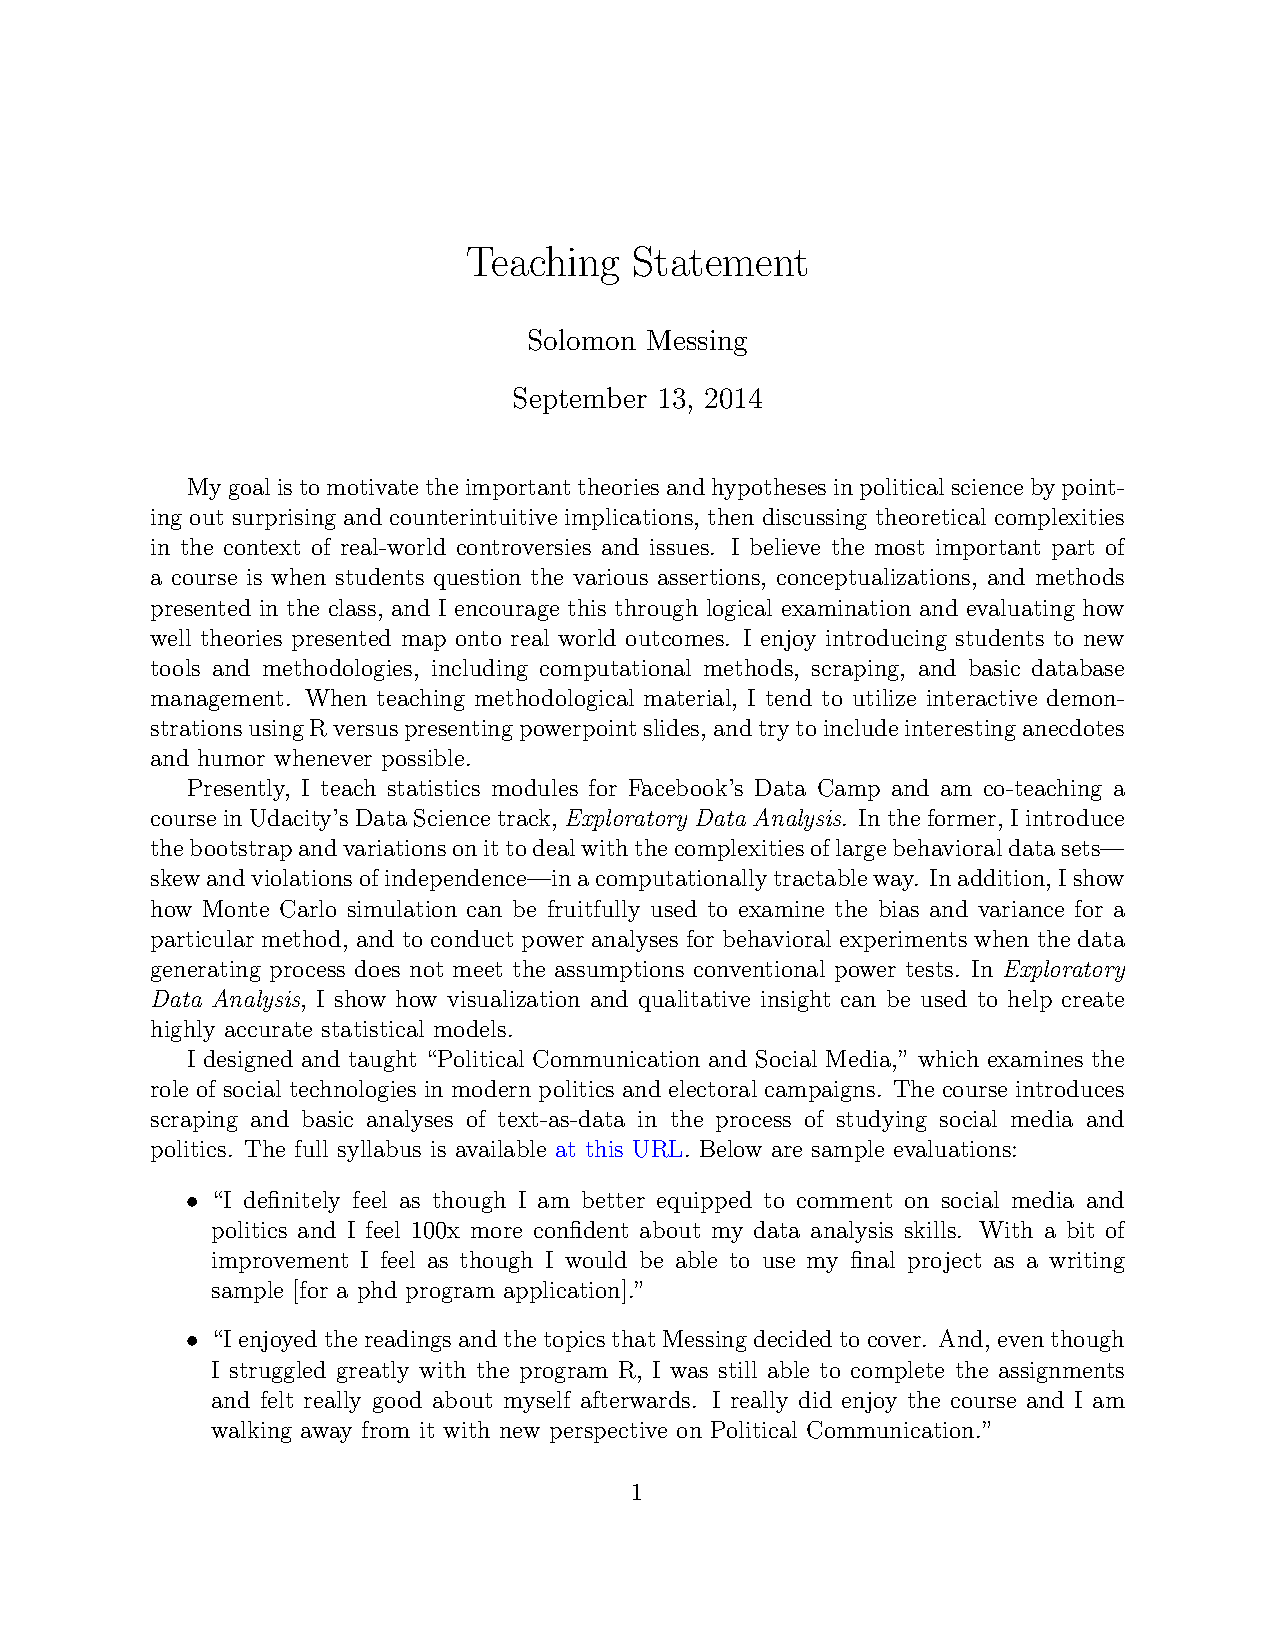
\includepdf[pages={-}]{TS.pdf}

\end{document}















